\documentclass{beamer}
\usetheme{metropolis}
%\setbeamersize{text margin left=.2cm,text margin right=.2cm}
\usepackage{graphicx}
\graphicspath{{../../images/}}
%\usepackage[french]{babel}
%\usepackage{listings}
%\usepackage{lipsum}
\usepackage{boolexpr}
\usepackage{kpfonts}
\usepackage{caption}
\usepackage{wrapfig}
\usepackage{tkz-graph}
\usepackage{tikz}
%\usepackage{chngcntr}
\usepackage[labelformat=empty]{caption}
\usepackage[official]{eurosym}

\usepackage{minted}

\usepackage{siunitx}

% http://tex.stackexchange.com/questions/114830/how-can-i-use-lvert-and-rvert-norm-symbols-x-with-the-iwona-math-font
\usepackage[math]{iwona}
\usepackage{scalerel}
\def\lVert{\mid\!\mid}
\def\rVert{\mid\!\mid}

\usepackage[normalem]{ulem}
%\newcommand{\Adj}{\mathbf{A}}
\usepackage{mathtools}

\usepackage{../../custom}
\usepackage{amsfonts}
%\newcommand{\jsrcodepath}{../../code}
%\usepackage{jsr}

\newcommand{\expe}[2]{\la #1, #2 \ra}

\usepackage{framed}

%\usepackage{mathtools,xparse}
%\DeclarePairedDelimiter{\norm}{\lVert}{\rVert}
\newcommand\Wider[2][3em]{%
\makebox[\linewidth][c]{%
  \begin{minipage}{\dimexpr\textwidth+#1\relax}
  \raggedright#2
  \end{minipage}%
  }%
}

\newcommand{\aeur}{\alpha_\text{\euro}}
\newcommand{\adol}{\alpha_\$}
\newcommand{\apou}{\alpha_\text{\pounds}}

\title{Polynomial and Moment Optimization in Julia and JuMP}
\date{August 24, 2019}
\author{Beno\^it Legat (UCLouvain)}
%\institute{Los Alamos National Laboratory, 16th July 2019}
%\institute{UCLouvain\\
%           Massachusetts Institute of Technology (MIT)\\
%           Rice University\\
%           Los Alamos National Laboratory (LANL)}

% https://tex.stackexchange.com/questions/426088/texlive-pretest-2018-beamer-and-subfig-collide
\makeatletter
\let\@@magyar@captionfix\relax
\makeatother
\begin{document}
  \maketitle

  \begin{frame}
    \tableofcontents
  \end{frame}

\section{Motivation}

  \begin{frame}[fragile]
    \frametitle{MathOptInterface (MOI)}
    MOI in a nutshell:
    \begin{itemize}
      \item \verb|add_variable(model)|.
      \item \verb|add_constraint(model, func, set)|, e.g. $2x + 3y = 1$ $\to$ (\verb|2*x + 3*y|)-in-\verb|EqualTo(1.0)|.
      \item \verb|set|, \verb|get| attributes, e.g., \verb|ObjectiveSense|, \verb|ObjectiveFunction|.
    \end{itemize}
    Extensible framework:
    \begin{itemize}
      \item \alert{Generic} on attribute, function and set types. New ones can be defined \alert{independently}.
      \item Solver-\alert{specific} features easily exposed to JuMP/MOI users through \alert{custom} attributes.
      \item Expose \alert{specialized} problem structure easily through \alert{custom} functions, sets (e.g. Sum-of-Squares variables/constraints).
    \end{itemize}
  \end{frame}

  \begin{frame}{Semidefinite programming}
    \begin{align*}
      \mini_{Q \in \SymK} \quad & \la C, Q \ra & \maxi_{y \in \R^n} \quad & \la b, y \ra\\
      \subtoq & \la A_i, Q \ra = b_i & \subtoq & \sum_i A_i y_i \preceq C\\
        & Q \succeq 0
    \end{align*}
    \textbf{File format}: SDPA

    \textbf{Solvers}: CSDP, SDPA, DSDP, SDPLR, ...

    \textbf{Variables}: $Q$ block diagonal, nonnegative scalar variables ($1 \times 1$ blocks) or SDP matrices.

    \textbf{Constraints}: Affine equations.
  \end{frame}

  \begin{frame}[fragile]
    \frametitle{Conic Modelling}
\begin{minted}{Julia}
using JuMP
model = Model(...)
@variable(model, -1 <= x <= 1)
@variable(model, y)
@variable(model, z <= 0)
@constraint(model, [x + y x
                    y     x - y] in PSDCone())
@constraint(model, [x + y, z, y] in SecondOrderCone())
@objective(model, x^2 - 2x*z + z^2)
\end{minted}
  \end{frame}

  \begin{frame}
    \frametitle{The gap between models and solvers}
    The solver interface should only support structures and the algorithm \alert{exploits}:
    \begin{itemize}
      \item
        $n$ solvers and $m$ structures $\to$ $mn$ transformations $\to$ \alert{unscalable} for large $m, n$.
      \item
        enables \alert{evaluation} of formulation \alert{quality}, e.g. automatic transformation and
        automatic dualization.
    \end{itemize}

    The model should
    \begin{itemize}
      \item be \alert{independent} from solvers.
      \item represent the structure \alert{exploitable} by algorithms.
      \item allow reprentable structure \alert{unknown} to solvers, e.g. Sum-of-Squares variables/constraints.
    \end{itemize}
  \end{frame}

  \begin{frame}
    \frametitle{Bridging the gap}
    \[ x \in S_1 \Leftrightarrow Ax \in S_2 \qquad AS_1 = S_2 \]
    \[ A^* y \in S_1^* \Leftrightarrow y \in S_2^* \qquad S_1^* = A^* S_2^* \]
    In Lagrangian:
    \[ \langle Ax, y \rangle_2 = \langle x, A^* y \rangle_1 \]
    \vspace{-0.5cm}
    \begin{block}{Transformation of variable-in-$S_2$ to variable-in-$S_1$.}
%      \[ Ax \in S_1 \Leftrightarrow x \in S_2 \qquad S_1 = AS_2 \]
%      \[ y \in S_1^* \Leftrightarrow A^* y \in S_2^* \qquad A^* S_1^* = S_2^* \]
%
%      Dans un Lagrangien:
%      \[ \langle x, A^* y \rangle_2 = \langle A x, y \rangle_1 \]
      \begin{enumerate}
        \item[Primal] Transform value $v$ to $Av$.
        \item[Dual] Transform dual $y$ to $A^{-*}y$.
      \end{enumerate}
    \end{block}
    \begin{block}{Transformation of $f$-in-$S_1$ constraint to $Af$-in-$S_2$ constraint.}
      %Transforme constraint $f$-in-$S_1$ en $Af$-in-$S_2$.

      \begin{enumerate}
        \item[Primal] Transform value $v$ of $Af$ to $A^{-1}v$ of $f$.
        \item[Dual] Transform dual $y$ of $A^*y$.
      \end{enumerate}
    \end{block}
  \end{frame}

\section{Examples}

  \begin{frame}[allowframebreaks]
    \frametitle{Examples}
    \begin{block}{FlipSignBridge}
      \begin{itemize}
        \item \textbf{Variable} $x \ge l$ substituted by $x = -y$ where $y \le -l$.
        \item \textbf{Constraint} $a^\top x \le \beta$ transformed into $-a^\top x \ge -\beta$.
      \end{itemize}
    \end{block}
    \begin{block}{VectorizeBridge}
      \begin{itemize}
        \item \textbf{Variable} $x \ge l$ substituted by $x = y + l$ where $y \in \R^1_+$.
        \item \textbf{Constraint} $a^\top x \le \beta$ transformed into $[a^\top x - \beta] \in \R^1_-$.
      \end{itemize}
    \end{block}
    \begin{block}{IntervalBridge}
      \begin{itemize}
        \item \textbf{Constraint} $l \le a^\top x \le u$ transformed into $a^\top x \ge l$ and $a^\top x \le u$.
      \end{itemize}
    \end{block}
    \begin{block}{IndicatorBridge}
      \begin{itemize}
        \item \textbf{Constraint} $y$ binary, $\neg y \Rightarrow a^\top x \le \beta$ transformed into $z$ binary, $z + y = 1$ and $z \Rightarrow a^\top x \le \beta$.
      \end{itemize}
    \end{block}
%    \begin{block}{ZerosBridge}
%      \begin{itemize}
%        \item \textbf{Variable} $x \in \{\mathbf{0}_n\}$ transformée en $x = \mathbf{0}_{n \times 0}y$ pour $y \in \R^0$.
%      \end{itemize}
%    \end{block}
    \begin{block}{FreeBridge}
      \begin{itemize}
        \item \textbf{Variable} $x \in \R$ substituted by $x = y + z$ where $y \in \R_+$ and $z \in \R_-$.
      \end{itemize}
    \end{block}

    \begin{block}{SlackBridge}
      \begin{itemize}
        \item \textbf{Constraint} $f \in S$ transformed into $f = x$ for variable $x \in S$.
        \item \textbf{Objective} $\min f$ transformed into $\min x$ with $f \le x$.
      \end{itemize}
    \end{block}
  \end{frame}

\begin{frame}{RSOC to PSD}
  Transforms rotated second order cone into positive semidefinite cone.
  By Schur Complement: $\lVert x\rVert_2^2 < 2tu, t, u > 0$ iff
  $$
  \begin{cases}
    u > 0\\
    2tu > x^\top x
  \end{cases}
  \Leftrightarrow
  \begin{cases}
    uI \succ 0\\
    t - x^\top (2uI)^{-1} x \succ 0
  \end{cases}
  \Leftrightarrow
  \begin{pmatrix}
    t & x^\top\\
    x & 2uI
  \end{pmatrix} \succ 0.
  $$
  \begin{block}{Dual of $u$}
    Diagonal at $(2,2), (3, 3), \ldots, (n, n)$ is $2u \mathbf{1}$ so
    dual of $u$ is scalar product between $(2\mathbf{1})^\top$ and dual of
    diagonal at $(2,2), (3, 3), \ldots, (n, n)$.
  \end{block}
  \begin{block}{Dual of $x$}
    Twice dual of $(1, 2), (1, 3), \ldots, (1, n)$.
    Pay attention to scalar product of vectorized PSD cone.
  \end{block}
\end{frame}

\begin{frame}{Quadratic to RSOC}
  Transforms quadratic constraints into rotated second order cone constraints.
  $$\frac{1}{2}x^T Q x + a^T x + \beta \le 0$$
  $Q$ PSD $\to$ Cholesky $Q = U^\top U$:
  $$\lVert U x\rVert_2^2 \le 2 (-a^T x - \beta)$$
  so $(1, -a^T x - \beta, Ux) \in {}$ RSOC.
\end{frame}

\begin{frame}{Second order cone and complementarity slackness}
  If $(t, x), (u, y) \in {}$ SOC and $(t, x) \cdot (u, y) = 0$,
  then $(u, y)$ is parallel to $(t, -x)$ or $(t, x)$ is zero or $(u, y)$ is zero.
  \begin{center}
    \begin{tikzpicture}[scale=2]
      \draw[->] (0, -0.1) to (0, 1.5);
      \node[right] at (0, 1.5) {$t, u$};
      \draw[->] (-1.5, 0) to (1.5, 0);
      \node[above] at (1.5, 0) {$x, y$};
      \draw[dashed] (0, 0) to (1.4, 1.4);
      \draw[->] (0, 0) to (1, 1);
      \draw[dashed] (0, 0) to (-1.4, 1.4);
      \draw[->] (0, 0) to (-1, 1);
      \draw (0.1, 0.1) to (0, 0.2) to (-0.1, 0.1);
    \end{tikzpicture}
  \end{center}
\end{frame}

\begin{frame}{Lemma}
  If $(1, s, x), (v, u, y) \in {}$ RSOC and
  $(1, s, x) \cdot (v, u, y) = 0$, then
  $y = -ux$ and $v = u \lVert x \rVert_2^2/2$.

  \begin{block}{Proof (sketch)}
    \begin{align*}
      0 & = (1, s, x) \cdot (v, u, y)\\
      & = v + s u + x \cdot y\\
      \text{(Cauchy-Schwarz)} & \ge
      v + s u - \lVert x\lVert_2 \lVert y\lVert_2\\
      \text{(RotatedSOC)} & \ge
      v + s u - 2 \sqrt{s u  v}\\
      \text{(AM-GM)} & \ge
      v + s  u - 2  \frac{v + s u}{2}\\
      & = 0.
    \end{align*}
    See MOI QuadtoSOCBridge for details.
%    By assumption, the left-hand side is zero, hence all inequalities
%    are equalities. By Cauchy-Schwarz, this means that ∃σ ≥ 0 such
%    that `y = -σ*x`. By AM-GM, we have `v = s * u`.
%    By RotatedSOC, we have either:
%    1) `||y||_2^2 < 2 * u * v` and `||x||_2^2 = 2 * s = 0`: That implies
%       that `v = 0 * u = 0` hence `||y||_2^2 < 0` which is impossible.
%    2) `||x||_2^2 < 2 * s` and `||y||_2^2 = 2 * u * v = 0`: we have either:
%       a) `u = 0`: hence `v = s * u = 0` or
%       b) `v = 0`: since `s > 0`, `u = v / s = 0`.
%       In any case, `y = 0` and `u = v = 0` hence the statement holds.
%    3) `||x||_2^2 = 2 * s` and `||y||_2^2 = 2 * u * v`: we have
%       `σ^2 * ||x||_2^2 = ||y||_2^2 = 2 * u * v = 2 * u^2 * s` hence
%       `u = σ`. It follows that at `v = s * u = σ * ||x||_2^2/2`.         □
  \end{block}
\end{frame}

\begin{frame}{Quadratic to RSOC duals}
  Consider $z^T U^\top U z/2 + a^\top z + \beta \le 0$ transformed,
  so $(1, -a^T z - \beta, Uz) = (1, s, x) \in {}$ RSOC.

  RSOC in Lagrangian:
  \begin{align*}
    (1, s, x) \cdot (v, u, y)
    & = u (1, s, x) \cdot (\lVert x \rVert_2^2/2, 1, -x)\\
    & = u (\lVert x \rVert_2^2/2 + s - \lVert x \rVert_2^2)\\
    & = u (-\lVert x \rVert_2^2/2 + s)\\
    & = u (-\lVert Uz \rVert_2^2/2 - a^\top z - \beta)\\
    & = -u (z^T U^\top U z/2 + a^\top z + \beta)
  \end{align*}
  So the dual of the quadratic constraint is $-u$.
\end{frame}

\section{Combining bridges}

\begin{frame}{Interval constraint for SDPA}
\Wider[4em]{
  \begin{center}
    \begin{tikzpicture}[xscale=4.5, yscale=2]
      \tikzset{VertexStyle/.style = {}}
      \Vertex[x=1, y=-1, L={$a^\top x + \beta \ge l$}]{G}
      \Vertex[x=2, y=-1, L={$a^\top x + \beta \le u$}]{L}
      \Vertex[x=1, y=-2, L={$A x + b \in \mathbb{R}_+^1$}]{N}
      \Vertex[x=2, y=-2, L={$A x + b \in \mathbb{R}_-^1$}]{P}
      \Vertex[x=1, y=-3, L={$A x + b \in \{0\}^1$}]{Z}
      \Vertex[x=0, y=0, L={$x \le u$}]{VL}
      \Vertex[x=0, y=-1, L={$x \ge l$}]{VG}
      \Vertex[x=0, y=-2, L={$x \in \mathbb{R}_-^1$}]{VP}
      \tikzset{VertexStyle/.style = {
        shape = rectangle,
        draw
      }}
      \Vertex[x=1, y=0, L={$l \le a^\top x + \beta \le u$}]{I}
      \tikzset{VertexStyle/.style = {
        shape = rounded rectangle,
        draw
      }}
      \Vertex[x=2, y=-3, L={$a^\top x = \beta$}]{E}
      \Vertex[x=0, y=-3, L={$x \in \mathbb{R}_+^1$}]{VN}
      \tikzset{EdgeStyle/.style = {->}}
      \Edge[label={flip}](L)(G)
      \Edge[label={flip}](VP)(VN)
      \Edge[label={flip}](VL)(VG)
      \Edge[label={split}](I)(L)
      \Edge[label={split}](I)(G)
      \Edge[label={vectorize}](G)(N)
      \Edge[label={vectorize}](L)(P)
      \Edge[label={scalarize}](Z)(E)
      \Edge[label={slack}](P)(Z)
      \Edge[label={slack}](N)(Z)
      \Edge[label={slack}](N)(VN)
      \Edge[label={slack}](G)(VG)
      \tikzset{EdgeStyle/.style = {->, pos=0.3}}
      \Edge[label={slack}](G)(E)
      \tikzset{EdgeStyle/.style = {->, bend left=22, pos=0.3}}
      \Edge[label={slack}](P)(VP)
      \tikzset{EdgeStyle/.style = {->, bend left=20, pos=0.7}}
      \Edge[label={vectorize}](VL)(VP)
      \tikzset{EdgeStyle/.style = {->, bend left=25, pos=0.8}}
      \Edge[label={slack}](L)(E)
      \tikzset{EdgeStyle/.style = {->, bend right=20, pos=0.3}}
      \Edge[label={vectorize}](VG)(VN)
      \tikzset{EdgeStyle/.style = {->, bend right=25}}
      \tikzset{EdgeStyle/.style = {->, bend right=60, pos=0.2}}
      \Edge[label={slack}](L)(VL)
      \tikzset{EdgeStyle/.style = {->}}
      \Edge[label={flip}](P)(N)
    \end{tikzpicture}
  \end{center}
}
\end{frame}

\begin{frame}{Quadratic objective for SDPA}
\Wider[4em]{
  \begin{center}
    \begin{tikzpicture}[xscale=4.5, yscale=2]
      \tikzset{VertexStyle/.style = {}}
      \Vertex[x=2, y=-1, L={$x^\top Q x/2 + a^\top x \le \beta$}]{L}
      \Vertex[x=1, y=-1, L={$Ax + b \in {}$RSOC}]{R}
      \Vertex[x=1, y=-2, L={$A x + b \in \mathbb{S}_+$}]{P}
      \Vertex[x=0, y=-2, L={$x \in {}$RSOC}]{VR}
      \Vertex[x=1, y=-3, L={$A x + b \in \{0\}^1$}]{Z}
      \Vertex[x=1, y=0, L={$x$ free}]{F}
      \Vertex[x=0, y=0, L={$x \in \mathbb{R}_-^1$}]{VP}
      \Vertex[x=2, y=-1.6, L={$\min x$}]{SV}
      \tikzset{VertexStyle/.style = {
        shape = rectangle,
        draw
      }}
      \Vertex[x=2, y=0, L={$\min x^\top Q x/2 + a^\top x + \beta$}]{Q}
      \tikzset{VertexStyle/.style = {
        shape = rounded rectangle,
        draw
      }}
      \Vertex[x=2, y=-3, L={$a^\top x = \beta$}]{E}
      \Vertex[x=2, y=-2.4, L={$\min a^\top x$}]{AF}
      \Vertex[x=0, y=-3, L={$x \in \mathbb{S}_+$}]{VPSD}
      \Vertex[x=0, y=-1, L={$x \in \mathbb{R}_+^1$}]{VN}
      \tikzset{EdgeStyle/.style = {->}}
      %\Edge[label={flip}](L)(G)
      %\Edge[label={flip}](VP)(VN)
      %\Edge[label={flip}](VL)(VG)
      %\Edge[label={split}](I)(L)
      %\Edge[label={split}](I)(G)
      %\Edge[label={vectorize}](G)(N)
      \Edge[label={slack}](Q)(L)
      \Edge[label={slack}](Q)(F)
      \Edge[label={quad}](L)(R)
      \Edge[label={slack}](P)(Z)
      \Edge[label={slack}](P)(VPSD)
      \Edge[label={slack}](R)(VR)
      \Edge[label={scalarize}](Z)(E)
      \Edge[label={rsoctopsd}](R)(P)
      \Edge[label={rsoctopsd}](VR)(VPSD)
      \Edge[label={free}](F)(VP)
      \Edge[label={free}](F)(VN)
      \Edge[label={flip}](VP)(VN)
      \Edge[label={functionize}](SV)(AF)
      \tikzset{EdgeStyle/.style = {->, bend left=30, pos=0.7}}
      \Edge[label={slack}](R)(Z)
      \tikzset{EdgeStyle/.style = {->, bend left=45, pos=0.85}}
      \Edge[label={slack}](Q)(SV)
    \end{tikzpicture}
  \end{center}
}
\end{frame}

\section{Automatic selection of bridges}

%\begin{frame}
%  \frametitle{Selection of bridges}
%  How to select bridges \alert{automatically} ?
%
%  \begin{block}{Example}
%    Free variable for SDP solver:
%    \begin{itemize}
%      \item FreeBridge: $x \in \R$ $\to$ $y \in \R_+$ (supported) and $z \in \R_-$ (\alert{not} supported)
%      \item FlipSignBridge: $x \in \R_-$ $\to$ $y \in \R_+$.
%    \end{itemize}
%  \end{block}
%
%  Shortest path ?
%\end{frame}


\begin{frame}
  \frametitle{Shortest path in directed Hypergraph}
  \vspace{-.2cm}
  \begin{block}{Nodes}
    Node for each set $S$ (variable-in-$S$).

    Node for each constraint $F$-in-$S$.

    Node for each objective function $F$.

    Types $F$ and $S$ are \alert{not limited} to those defined in MOI.

    \alert{Infinitely} many nodes, we need to be \alert{lazy}.
  \end{block}
  \vspace{-.2cm}
  \begin{block}{Edges}
    Each bridge defined possible \alert{infinitely} many edges.

    For each edge and ingoing node: outgoing nodes are
    \begin{itemize}
        \item variable-in-$S$ created.
        \item constraints $F$-in-$S$ created.
        \item objective $F$ set.
    \end{itemize}
  \end{block}
  %\vspace{-.2cm}

  %Solved by a modified \alert{Bellman-Ford} algorithm.
\end{frame}

\begin{frame}
  \frametitle{Shortest Path Problem}
  Need to solve
  \begin{align*}
    d_\mathcal{V}(S) & =
    1 + \min_{B \in \mathcal{B}_\mathcal{V}(S)}
		\sum_{S' \in \mathcal{A_\mathcal{V}}(B, S)} d_\mathcal{V}(S') +
	  \sum_{(F', S') \in \mathcal{A_\mathcal{C}}(B, S)} d_\mathcal{C}(F', S')\\
    d_\mathcal{C}(F, S) & =
    1 + \min_{B \in \mathcal{B}_\mathcal{C}(F, S)}
		\sum_{S' \in \mathcal{A_\mathcal{V}}(B, F, S)} d_\mathcal{V}(S') +
	  \sum_{(F', S') \in \mathcal{A_\mathcal{C}}(B, F, S)} d_\mathcal{C}(F', S')\\
    d_\mathcal{O}(F) & =
    1 + \min_{B \in \mathcal{B}_\mathcal{O}(F)}
		\sum_{S' \in \mathcal{A_\mathcal{V}}(B, F)} d_\mathcal{V}(S') +
	  \sum_{(F', S') \in \mathcal{A_\mathcal{C}}(B, F)} d_\mathcal{C}(F', S')\\
    & \quad + d_\mathcal{O}(\mathcal{A_\mathcal{O}}(B, F))
  \end{align*}
  with
	\begin{itemize}
		\item $d_\mathcal{V}(S) = 0$ if constrained variables in $S$ supported by optimizer.
		\item $d_\mathcal{C}(F, S) = 0$ if $F$-in-$S$ constraints supported by optimizer.
		\item $d_\mathcal{O}(F) = 0$ if objective function $F$ supported by the optimizer.
	\end{itemize}
\end{frame}

\begin{frame}
  \frametitle{Shortest path algrithms ?}
  \begin{itemize}
    \item Breath-First Search : For edges with cost 1
    \item Dijkstra : For edges with nonnegative cost
    \item Bellman-Ford : For edges with any real cost (+ negative cycles)
  \end{itemize}

  Choice: a modified \emph{Bellman-Ford algorithm}.
\end{frame}

\begin{frame}[fragile]
  \frametitle{Classical Bellman-Ford algorithm}
  \begin{itemize}
    \item \texttt{N}: set of nodes
    \item \texttt{E}: set of edges
    \item \texttt{d}: distance
    \item \texttt{b}: next node
  \end{itemize}
\begin{minted}{Julia}
for _ in 1:length(N)-1:
  for each edge u=>v with weight w in E
    if d[u] + w < d[v]:
      d[v] = d[u] + w
      b[v] = u
    end
  end
end
\end{minted}
Complexity $\mathcal{O}(|N| \cdot |E|)$
\end{frame}

\begin{frame}
  \frametitle{Target constraint types}
  \textbf{Invariant}: $d_\mathcal{V}$, $d_\mathcal{C}$, $d_\mathcal{O}$
  are correct when defined.

	\begin{block}{constrained variable in $S$ added by user}
		$\to$ generate  $\mathcal{V}$ (resp. $\mathcal{C}$): list of needed new entries
		to compute in $d_\mathcal{V}$ (resp. $d_\mathcal{C}$).
	\end{block}

	\begin{block}{$F$-in-$S$ constraint added by user}
		$\to$ generate  $\mathcal{V}$ (resp. $\mathcal{C}$): list of needed new entries
		to compute in $d_\mathcal{V}$ (resp. $d_\mathcal{C}$).
	\end{block}

	\begin{block}{Objective function $F$ constraint added by user}
		$\to$ generate  $\mathcal{V}$ (resp. $\mathcal{C}$, $\mathcal{O}$): list of needed new entries
		to compute in $d_\mathcal{V}$ (resp. $d_\mathcal{C}$, $d_\mathcal{O}$).
	\end{block}

\end{frame}

\begin{frame}{Add target variable type}
  \begin{algorithm}[H]
    \caption{recursive add $S$}
    \begin{algorithmic}
      \STATE add $S$ to $\mathcal{V}$
      \FOR{$B \in \mathcal{B}_\mathcal{V}(S)$}
        \FOR{$S' \in \mathcal{A}_\mathcal{V}(B, S)$}
          \IF{$d_\mathcal{V}(S')$ not defined}
            \STATE recursive add $S'$
          \ENDIF
        \ENDFOR
        \FOR{$(F', S') \in \mathcal{A}_\mathcal{C}(B, S)$}
          \IF{$d_\mathcal{C}(F', S')$ not defined}
            \STATE recursive add $F'$-in-$S'$
          \ENDIF
        \ENDFOR
      \ENDFOR
    \end{algorithmic}
  \end{algorithm}
\end{frame}

\begin{frame}{Add target constraint type}
  \begin{algorithm}[H]
    \caption{recursive add $F$-in-$S$}
    \begin{algorithmic}
      \STATE add $F$-in-$S$ to $\mathcal{C}$
      \FOR{$B \in \mathcal{B}_\mathcal{C}(F, S)$}
        \FOR{$S' \in \mathcal{A}_\mathcal{V}(B, F, S)$}
          \IF{$d_\mathcal{V}(S')$ not defined}
            \STATE recursive add $S'$
          \ENDIF
        \ENDFOR
        \FOR{$(F', S') \in \mathcal{A}_\mathcal{C}(B, F, S)$}
          \IF{$d_\mathcal{C}(F', S')$ not defined}
            \STATE recursive add $F'$-in-$S'$
          \ENDIF
        \ENDFOR
      \ENDFOR
    \end{algorithmic}
  \end{algorithm}
\end{frame}

\begin{frame}
  \frametitle{Modified Bellman-Ford algorithm}
  \begin{algorithmic}
    \WHILE{$d_\mathcal{V}$ or $d_\mathcal{C}$ changed}
      \FOR{$S \in \mathcal{V}$, $B \in \mathcal{B}_\mathcal{V}(S)$}
				\STATE $u \leftarrow 1 + \sum_{S' \in \mathcal{A}_\mathcal{V}(B, S)} d_\mathcal{V}(S') + \sum_{(F', S') \in \mathcal{A}_\mathcal{C}(B, S)} d_\mathcal{C}(F', S')$
				\IF{$u < d_\mathcal{V}(S)$}
					\STATE $d_\mathcal{V}(S) \leftarrow u$
				\ENDIF
      \ENDFOR
      \FOR{$F$-in-$S \in \mathcal{C}$, $B \in \mathcal{B}_\mathcal{C}(F, S)$}
				\STATE $u \leftarrow 1 + \sum_{S' \in \mathcal{A}_\mathcal{V}(B, F, S)} d_\mathcal{V}(S') + \sum_{(F', S') \in \mathcal{A}_\mathcal{C}(B, F, S)} d_\mathcal{C}(F', S')$
				\IF{$u < d_\mathcal{C}(F, S)$}
					\STATE $d_\mathcal{C}(F, S) \leftarrow u$
				\ENDIF
      \ENDFOR
    \ENDWHILE
  \end{algorithmic}
\end{frame}

\section{Integration with JuMP}

\begin{frame}[fragile]
  \frametitle{Extending JuMP macros}
\begin{minted}{Julia}
@constraint(model, [x + 1, x - y] in MOI.Zeros())
\end{minted}
  Implementation:
\begin{minted}{Julia}
function build_constraint(
    _error::Function,
    func::Vector{<:AbstractJuMPScalar},
    set::MOI.AbstractVectorSet)
    return VectorConstraint(x, set)
end
\end{minted}
\end{frame}

\begin{frame}[fragile]
  \frametitle{Extending JuMP macros: Custom set}
\begin{minted}{Julia}
@constraint(model, [x + 1, x - y] in SecondOrderCone())
\end{minted}
  Implementation:
\begin{minted}{Julia}
function build_constraint(_error::Function,
                          f::AbstractVector,
                          s::AbstractVectorSet)
    set = moi_set(s, length(f))
    return build_constraint(_error, f, set)
end
function moi_set(::SecondOrderCone, dim::Int)
  return MOI.SecondOrderCone(dim)
end
\end{minted}
\end{frame}

\begin{frame}[fragile]
  \frametitle{Extending JuMP macros: PSD cone}
\begin{minted}{Julia}
using LinearAlgebra # For Symmetric
@constraint(model, Symmetric([x + 1 x - y
                              x - y y]) in PSDCone())
\end{minted}
  Implementation:
\begin{minted}{Julia}
function build_constraint(_error::Function,
                          Q::Symmetric,
                          ::PSDCone)
    n = LinearAlgebra.checksquare(Q)
    func = [Q[i, j] for j in 1:n for i in 1:j]
    set = MOI.PositiveSemidefiniteConeTriangle(n)
    VectorConstraint(func, set,
                     SymmetricMatrixShape(n))
end
\end{minted}
\end{frame}

\section{Sum-of-Squares example}

  \begin{frame}{Nonnegative quadratic forms into sum of squares}
    \begin{tikzpicture}
      \draw[->, bend left=30] (-1, 1.6) node[left] {$(x_1, x_2, x_3)$} to (-.1, 1.3);
      \draw[->, bend left=30] (-1, 1.6) to (.9, 1.25);
      \draw[->, bend right=30] (2.1, 2) node[right] {\alert{unique}} to (1.55, 1.35);
      \node at (-.2, 1.2) {$p(x)$};
      \node at (.5, 1.2) {$=$};
      \node at (1.3, 1.2) {$x^\Tr Q x$};
      \node at (-2.4, 0) {$x_1^2 + 2x_1x_2 + 5x_2^2 + 4x_2x_3 + x_3^2$};
      \node at (.5, 0) {$=$};
      \node at (2.4, 0) {$x^\Tr \begin{pmatrix}1 & 1 & 0\\1 & 5 & 2\\ 0 & 2 & 1\end{pmatrix} x$};
      \node at (-1, -1.5) {$p(x) \geq 0$ $\forall x$};
      \node at (1.5, -1.5) {$Q \succeq 0$};
      \node at (.5, -1.5) {$\Longleftrightarrow$};
      \draw[->] (2.5, -1) to node[right] {cholesky} (2.5, -2.5);
      \node at (-3, -3.5) {$(x_1 + x_2)^2 + (2x_2 + x_3)^2$};
      \draw[->] (.2, -3.5) to (-.8, -3.5);
      \node at (3, -3.5) {$x^\Tr \begin{pmatrix}1 & 1 & 0\\0 & 2 & 1\end{pmatrix}^\Tr \begin{pmatrix}1 & 1 & 0\\0 & 2 & 1\end{pmatrix} x$};
    \end{tikzpicture}
  \end{frame}

  \begin{frame}{Nonnegative polynomial into sum of squares}
    \begin{tikzpicture}
      \draw[->, bend left=30] (-1, 1.6) node[left] {$(x_1, x_2, x_3)$} to (-.1, 1.3);
      \draw[->, bend left=20] (.6, 1.6) node[above] {$(x_1, x_1x_2, x_2)$} to (.9, 1.35);
      \draw[->, bend right=30] (2.1, 2) node[right] {\alert{\emph{not} unique}} to (1.55, 1.35);
      \node at (-.1, 1.2) {$p(x)$};
      \node at (.5, 1.2) {$=$};
      \node at (1.3, 1.2) {$X^\Tr Q X$};
      \node at (-2.5, 0) {$x_1^2 + 2x_1^2x_2 + 5x_1^2x_2^2 + 4x_1x_2^2 + x_2^2$};
      \node at (.5, 0) {$=$};
      \node at (2.3, 0) {$X^\Tr \begin{pmatrix}1 & 1 & 0\\1 & 5 & 2\\ 0 & 2 & 1\end{pmatrix} X$};
      \node at (-1, -1.5) {$p(x) \geq 0$ $\forall x$};
      \node at (1.5, -1.5) {$Q \succeq 0$};
      \node at (.5, -1.5) {$\Longleftarrow$};
      \draw[->] (2.5, -1) to node[right] {cholesky} (2.5, -2.5);
      \node at (-3, -3.5) {$(x_1 + x_1x_2)^2 + (2x_1x_2 + x_2)^2$};
      \draw[->] (.2, -3.5) to (-.6, -3.5);
      \node at (3, -3.5) {$X^\Tr \begin{pmatrix}1 & 1 & 0\\0 & 2 & 1\end{pmatrix}^\Tr \begin{pmatrix}1 & 1 & 0\\0 & 2 & 1\end{pmatrix} X$};
    \end{tikzpicture}
  \end{frame}

  \begin{frame}{When is nonnegativity equivalent to sum of squares ?}
    Determining whether a polynomial is nonnegative is \alert{NP-hard}.
    \begin{block}{Hilbert 1888}
      Nonnegativity of $p(x)$ of $n$ variables and degree $2d$ is equivalent to sum of squares in the following three cases:
      \begin{itemize}
        \item $n = 1$ : Univariate polynomials
        \item $2d = 2$ : Quadratic polynomials
        \item $n = 2$, $2d = 4$ : Bivariate quartics
      \end{itemize}
    \end{block}
    \begin{columns}
      \begin{column}{0.7\textwidth}
    \begin{block}{Motzkin 1967}
      First \alert{explicit} example:
      \[ x_1^4x_2^2 + x_1^2x_2^4 + 1 - 3x_1^2x_2^2 \geq 0 \quad \forall x \]
      but is \alert{not} a sum of squares.
    \end{block}
      \end{column}
      \begin{column}{0.3\textwidth}
        \centering
        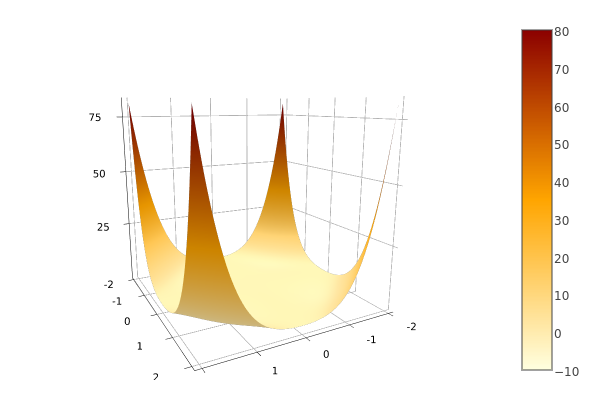
\includegraphics[trim=3cm .7cm 6cm 3cm, clip, width=\textwidth]{motzkin.png}
      \end{column}
    \end{columns}
  \end{frame}

\begin{frame}
  \frametitle{Sum-of-Squares bridges}
  Polynomial $p \in \Sigma$ ($p$ is SOS) iff
  $p = X^\top Q x$ with $Q \in \mathbb{S}_+$ ($Q$ is PSD).
  Hence $\Sigma = A \mathbb{S}_+$.

  SOSPolnomialBridge: Transformation of variable-in-$\Sigma$ to variable-in-$\mathbb{S}_+$.

  Transformation of contraint $F$-in-$\Sigma$: SlackBridge + SOSPolnomialBridge.
\end{frame}

\begin{frame}
  \frametitle{Result transformations}
  \begin{block}{Constraint Attribute}
    \textbf{Examples}: ConstraintPrimal, ConstraintDual, ConstraintFunction, ConstraintSet, ...

    \alert{Redirected} to bridge when constraint is bridged.
  \end{block}
  New attributes:
  \begin{itemize}
    \item GramMatrixAttribute: Gram matrix $Q$ indexed by $X$.
    \item MomentMatrixAttribute: Moment matrix index by $X$, dual of constraint $Q \in \mathbb{S}_+$.
    \item MomentsAttribute: Vector of moments, dual of constraint $p = X^\top Q X$.
  \end{itemize}
\end{frame}

\begin{frame}[fragile]
  \frametitle{Sum-of-Squares constraint macro}
\begin{minted}{Julia}
@constraint(model, p in SOSCone())
\end{minted}
  Implementation:
\begin{minted}{Julia}
function JuMP.build_constraint(_error::Function, p,
                               cone::SOSCone; kws...)
    coefs = coefficients(p)
    monos = monomials(p)
    set = JuMP.moi_set(cone, monos; kws...)
    shape = PolyJuMP.PolynomialShape(monos)
    return PolyJuMP.bridgeable(
        JuMP.VectorConstraint(coefs, set, shape),
        JuMP.moi_function_type(typeof(coefs)),
        typeof(set)
    )
end
\end{minted}
\end{frame}

\section{Reshaping}

\begin{frame}[fragile]
  \frametitle{Reshaping sets}
\begin{minted}{Julia}
function reshape_set(set::MOI.AbstractScalarSet,
                     ::ScalarShape)
    return set
end
function reshape_set(
    ::MOI.PositiveSemidefiniteConeTriangle,
    ::SymmetricMatrixShape
)
    return PSDCone()
end
\end{minted}
\end{frame}

\begin{frame}[fragile]
  \frametitle{Reshaping polynomial sets}
\begin{minted}{Julia}
function JuMP.reshape_set(set::SOSPolynomialSet,
                          ::PolyJuMP.PolynomialShape)
    return set.cone
end
\end{minted}
\end{frame}

\begin{frame}[fragile]
  \frametitle{Reshaping results}
\begin{minted}{Julia}
function reshape_vector(vectorized_form::Vector{T},
        shape::SymmetricMatrixShape) where T
    matrix = Matrix{T}(undef, shape.side_dimension,
                       shape.side_dimension)
    k = 0
    for j in 1:shape.side_dimension
        for i in 1:j
            k += 1
            matrix[j, i] = matrix[i, j] =
                vectorized_form[k]
        end
    end
    return Symmetric(matrix)
end
\end{minted}
\end{frame}

\begin{frame}[fragile]
  \frametitle{Reshaping polynomial results}
\begin{minted}{Julia}
function JuMP.reshape_set(set::SOSPolynomialSet,
                          ::PolyJuMP.PolynomialShape)
    return set.cone
end
function JuMP.reshape_vector(x::Vector,
                             shape::PolynomialShape)
    return polynomial(x, shape.monomials)
end
function JuMP.reshape_vector(x::Vector,
                             shape::MomentsShape)
    return measure(x, shape.monomials)
end
\end{minted}
\end{frame}

\begin{frame}[fragile]
  \frametitle{Dual shape}
  In JuMP:
\begin{minted}{Julia}
dual_shape(shape::AbstractShape) = shape
\end{minted}
  In PolyJuMP:
\begin{minted}{Julia}
function JuMP.dual_shape(shape::PolynomialShape)
    return MomentsShape(shape.monomials)
end
function JuMP.dual_shape(shape::MomentsShape)
    return PolynomialShape(shape.monomials)
end
\end{minted}
\end{frame}

\begin{frame}
  \frametitle{Conclusion}
  JuMP and MathOptInterface provide an optimization framework \alert{extensible} by \alert{design}.

  \vspace{4em}

  Bridges allow to communicate \alert{custom} structure to solvers from \alert{solver-independent} models.
\end{frame}

\end{document}
